% Notes on immersed boundary type method to solve the Eikonal Equation in 2D
\documentclass[11pt]{report}

\topmargin=0.0in
\oddsidemargin=0.0in
\evensidemargin=0.0in
\textwidth=6.5in
\marginparwidth=0.5in
\headheight=0pt
\textheight=9.0in

\usepackage{amsmath}
\usepackage{amsfonts}
\usepackage{geometry,color,graphicx}
\usepackage{subcaption}
\usepackage{hyperref}

\begin{document}
    \title{\textbf{Notes on implementing the Immersed Boundary Method to solve the Eikonal Equation in 2D}}
    \author{\textit{Balaje K \& Sanath Keshav}}
    \date{\today}
    \maketitle

\tableofcontents

\chapter{Eikonal equation in 2D}

The Eikonal equation in 2D is given by the following PDE
\begin{equation}
  |\nabla u| = 1
\end{equation}
where $u = u(x,y)$ in the 2D plane. Consider first a 2D rectangular domain, on which we first illustrate a Finite Difference Scheme to solve the Eikonal Equation. We start with the following boundary value problem.
\begin{eqnarray}
  |\nabla u| &=& 1 \;\;\;\; \text{in} \;\; \Omega := (-1,1) \times (-1,1)\\ \label{eq:1}
  u &=& 0 \;\;\;\; \text{on} \;\; \Gamma
\end{eqnarray}
where $\Gamma$ denotes the boundary of the rectangle under consideration.
\begin{figure}[h!]
  \centering
  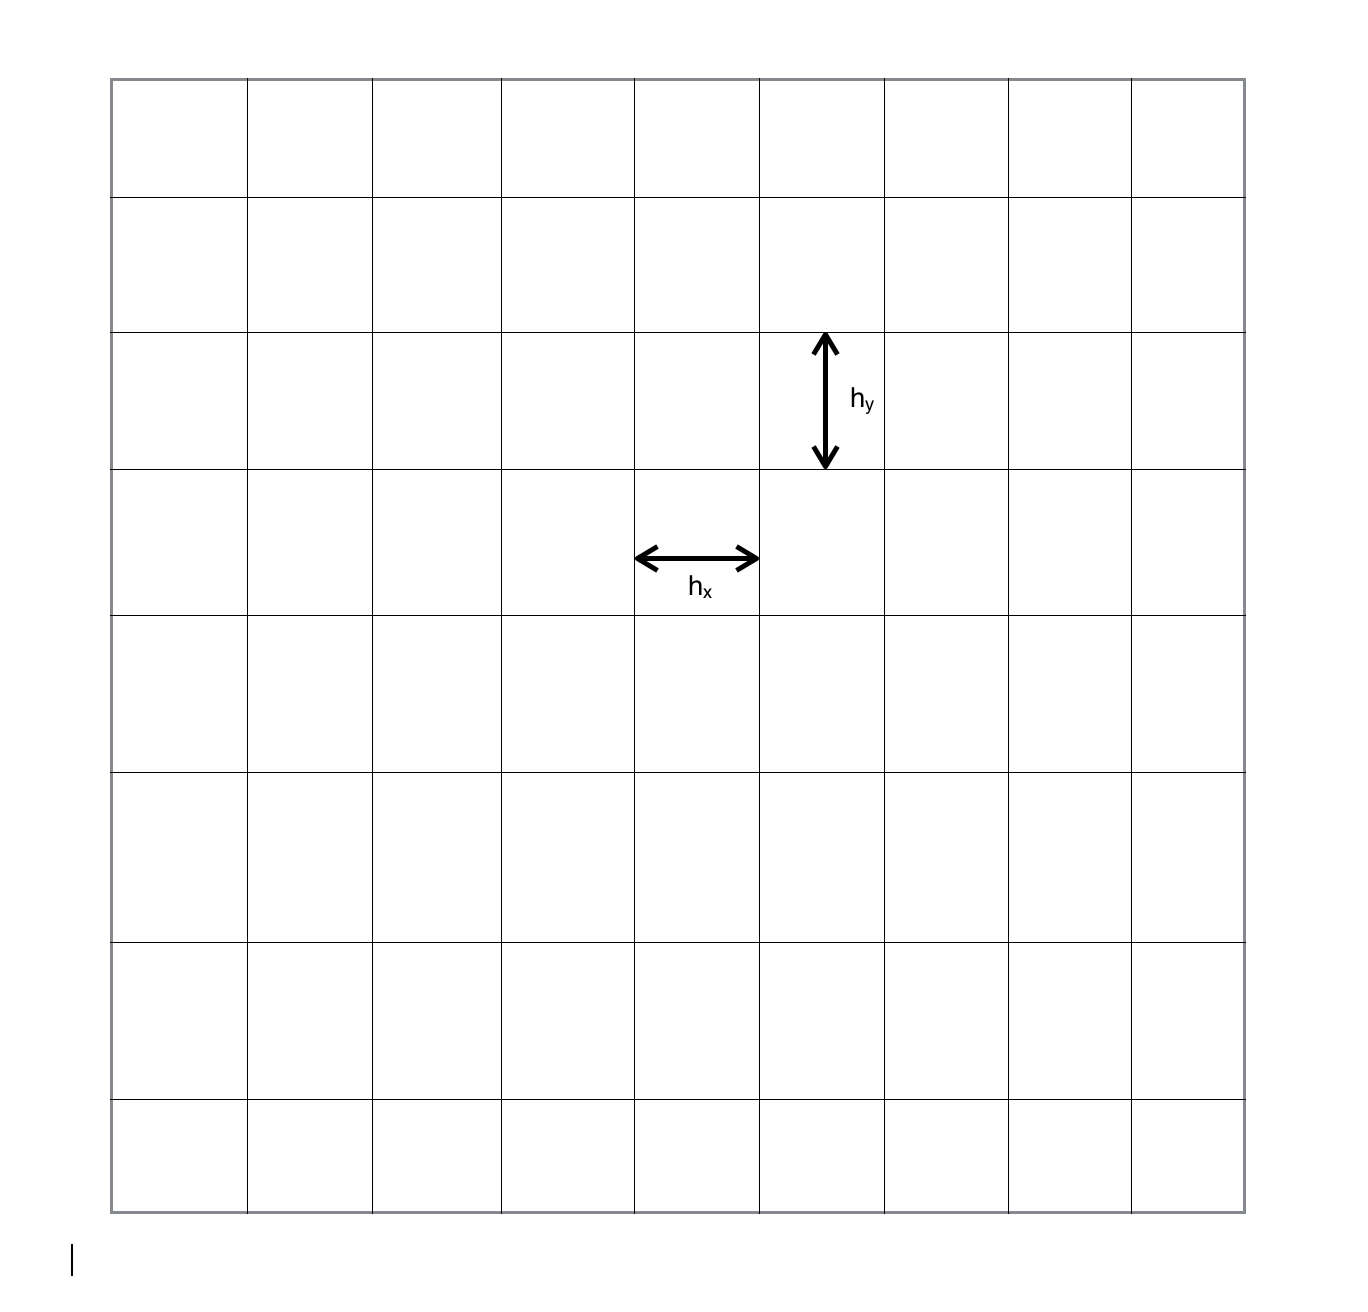
\includegraphics[scale=0.5]{rect.png}
  \caption{Rectangular Mesh}
  \label{fig:1}
\end{figure}\\

\noindent
First we take the PDE (\ref{eq:1}) and add a transient term $u_t$ to it. This makes it a time dependent problem. The idea is to solve this problem till it reaches the steady state. The corresponding initial boundary value problem is
\begin{eqnarray}
	u_t + |\nabla u| &=& 1 \;\;\;\; \text{in} \;\; (-1,1)\times(-1,1)\times(0,T] \\
	u(x,y,0) &=& 0 \;\;\;\; x,y \in \Omega\\
	u(x,y,t) &=& 0 \;\;\;\;  x,y \in \Gamma
\end{eqnarray}\\
\noindent
A finite difference mesh on a rectangle is shown in the following Figure \ref{fig:1}. The grid spacing along x-axis is given by $h_x$ and along y-axis  is given by $h_y$. A finite difference scheme due to Rouy and Tourin \cite{rouy} is  formulated below.\\

\noindent
Let 
\begin{eqnarray}
	h_x = \frac{2}{N_x}\\
	h_y = \frac{2}{N_y}
\end{eqnarray}
where $N_x$ and $N_y$ is the number of discretization along $x$ and $y$ directions respectively. Now $x_i = -1 + ih_x$ and $y_j = -1 + jh_y$ where $i = 1,2, \dots N_x-1$ and $j = 1,2, \dots N_y-1$.\\

\noindent
The time discretization, $\Delta t$, can be set using a suitable CFL Condition so that the solution does not diverge for large time steps. Let $u_{ij}^n$ denote the exact solution of the problem at the grid point $(x_i,y_j)$ and at time $t = n\Delta t$.\\

\noindent
Let $v_{ij}^n \approx u_{ij}^n$ at the grid point $(x_i,y_j)$. The scheme proposed by Rouy and Tourin to solve the Eikonal Equation is given by
\begin{eqnarray}\label{eq:2}
	v_{ij}^{n+1} &=& v_{ij}^n - \Delta t\left(\sqrt{D_x^2 + D_y^2}-1\right)\\ 
	D_x &=& max\left(\frac{v_{i+1,j}-v_{i,j}}{h_x},\frac{v_{i-1,j}-v_{i,j}}{h_x},0\right)\\
	D_y &=& max\left(\frac{v_{i,j+1}-v_{i,j}}{h_x},\frac{v_{i,j-1}-v_{i,j}}{h_x},0\right) \label{eq:3}
\end{eqnarray}\\

\noindent
It is shown in \cite{yong} that this scheme is consistent, stable, monotone and admits a comparison principle. Thus the scheme converges to a unique viscosity solution. \\

\noindent
The update formula is run till the steady state is achieved. That is, a preset tolerance $\epsilon$ such that $\lVert u^{n+1} - u^{n} \rVert < \epsilon$ must be satisfied so that the steady state is achieved. The results are shown in chapter 3.

\chapter{Immersed Boundary Method}
So far, the fintie difference techniques can be easily applied to a rectangular cartesian grid. The objective is to extend the same finite difference techniques to a variety other domains, for example - \textit{Circle, L-Domain, Circle with hole} etc. \\

\noindent
To illustrate the technique, we consider a circular domain. For comfort, let us consider a unit circle. We take a rectangular cartesian grid shown in Figure \ref{fig:1} and \textbf{``immerse"} the circluar domain into the rectangular mesh as shown in Figure \ref{fig:2}. This technique is known as the immersed boundary method \cite{pesk} which is widely used to solve problems in Fluid Mechanics.\\

\begin{figure}[h!]
	\centering
	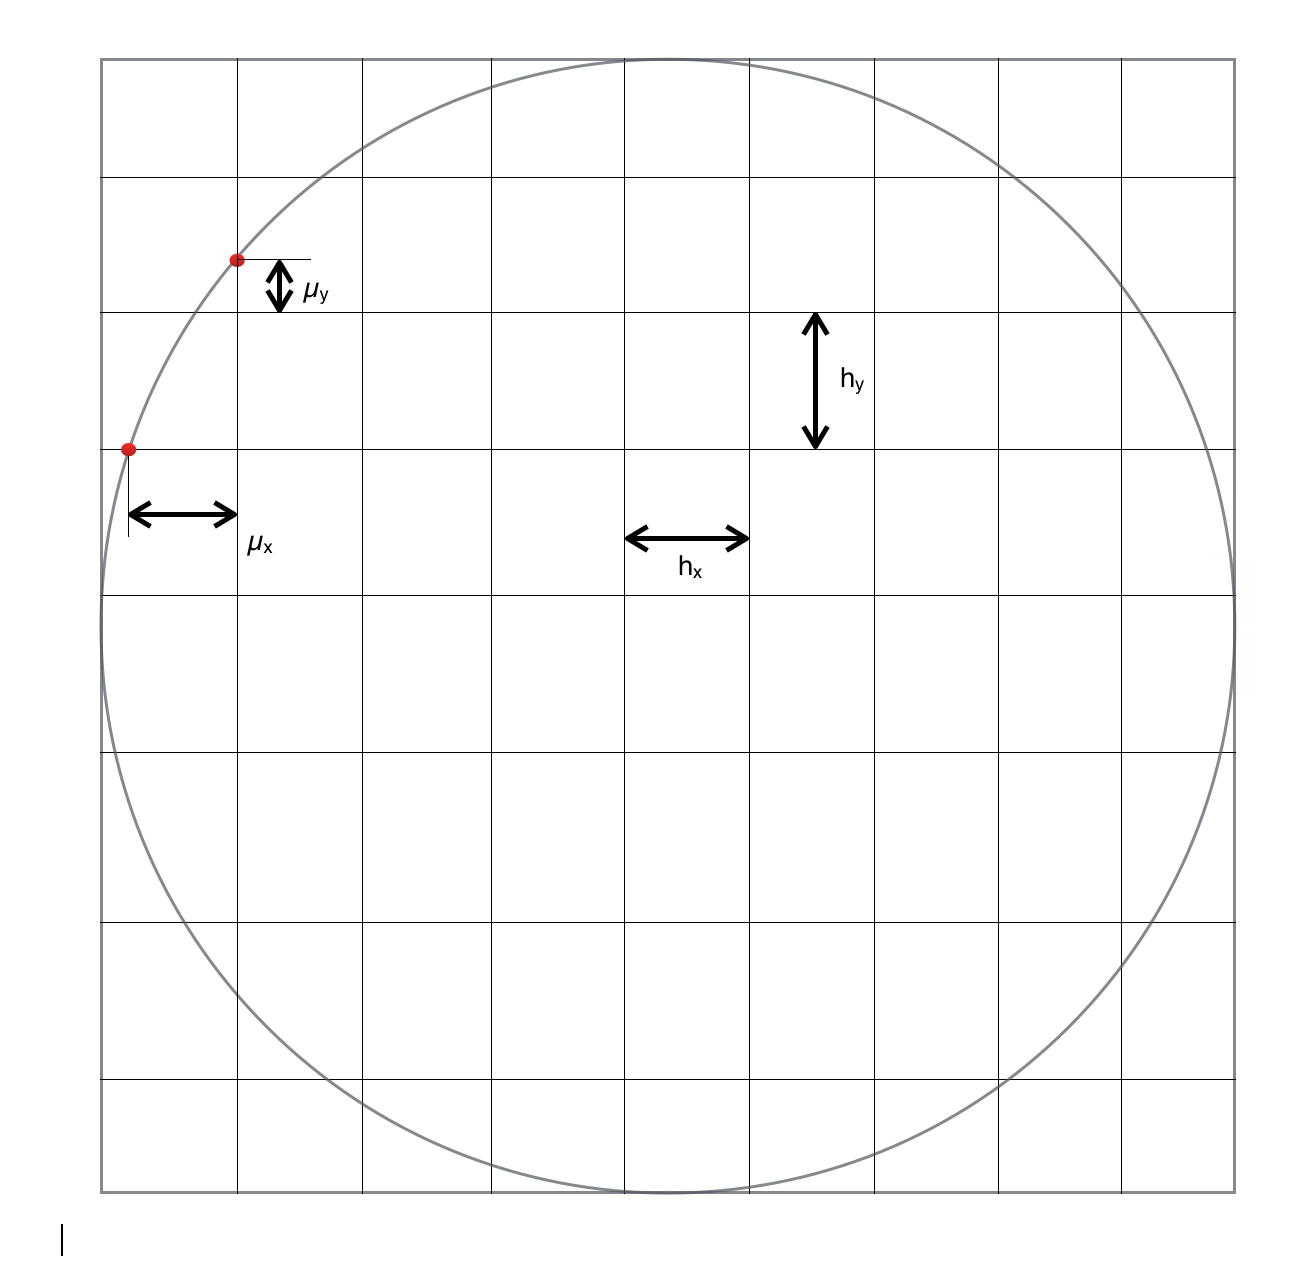
\includegraphics[scale=0.5]{circle-immerse.png}
	\caption{Immersed Circle}
	\label{fig:2}
\end{figure}

\noindent
The first challenge in this method is to track the interior and boundary of the 
immersed domain. For this we introduce a data structure called the \textbf{inout} matrix. The \textbf{inout} matrix is defined as follows,
\begin{equation}
	inout_{ij} = 
	\begin{Bmatrix}
	0, &\;\; \text{if} \;\; (x_i,y_j) \;\; \text{lies inside the immersed domain}\\
	1, &\;\; \text{otherwise}
	\end{Bmatrix}
\end{equation}.

\noindent
The way to track the boundary of the immersed domain using the \textbf{inout} matrix is natural. We simply ignore the grid points whose \textbf{inout} entry is $1$ and set the value $u(x,y) = 0$ at those places. We then solve the eikonal equation using (\ref{eq:2}) - (\ref{eq:3}) only inside the immersed boundary where the \textbf{inout} value is $0$.\\

\noindent
To apply the boundary conditions, we are in a position to obtain the points marked in \textbf{red} in Figure \ref{fig:2}. These points are easily obtained by solving the grid lines $x = -1 + ih_x$ or $y = -1 + jh_y$ with the equation of the circle. Note that, from the Dirichlet boundary condition, the value of $u(x,y)$ is prescribed in the problem at these points. \\

\noindent
When we apply the finite difference formula on the point which is immediately next to the \textbf{red} point - inside the domain, we are in a position to use the distances $\mu_x$ and $\mu_y$ to calculate the finite differences. This is the place where we choose to ignore the points outside the immersed boundary, and take the points that lie on the circle instead.\\

\noindent
With the distances $\mu_x$ and $\mu_y$, the update formula (\ref{eq:2})-(\ref{eq:3}) near the immersed boundary becomes,
\begin{eqnarray}
	v_{ij}^{n+1} &=& v_{ij}^n - \Delta t\left(\sqrt{D_x^2 + D_y^2}-1\right)\\ 
	D_x &=& max\left(\frac{v_{i+1,j}-v_{i,j}}{\mu_1},\frac{v_{i-1,j}-v_{i,j}}{\mu_2},0\right)\\
	D_y &=& max\left(\frac{v_{i,j+1}-v_{i,j}}{\mu_3},\frac{v_{i,j-1}-v_{i,j}}{\mu_4},0\right)
\end{eqnarray}
where $\mu_{1,\dots,4}$ is chosen accordingly, depending on the position of top, bottom, left or right neighboring grid points. If the grid point above the current point, lies on the boundary, then $\mu_3 = \mu_y$ and $\mu_1 =  \mu_2 = h_x, \;\; \mu_4 = h_y$ and so on. There may be cases where two of the neighboring grid points may lie on the boundary. All those cases must be taken proper care of. Results of some numerical experiments are shown in the next chapter.

\chapter{Results}
Some Numerical Experiments were carried out using the Rouy and Tourin scheme for a variety of domains. First we illustrate the solution using a simple rectangular (a square rather) domain.
\begin{figure}[h!]
	\centering
	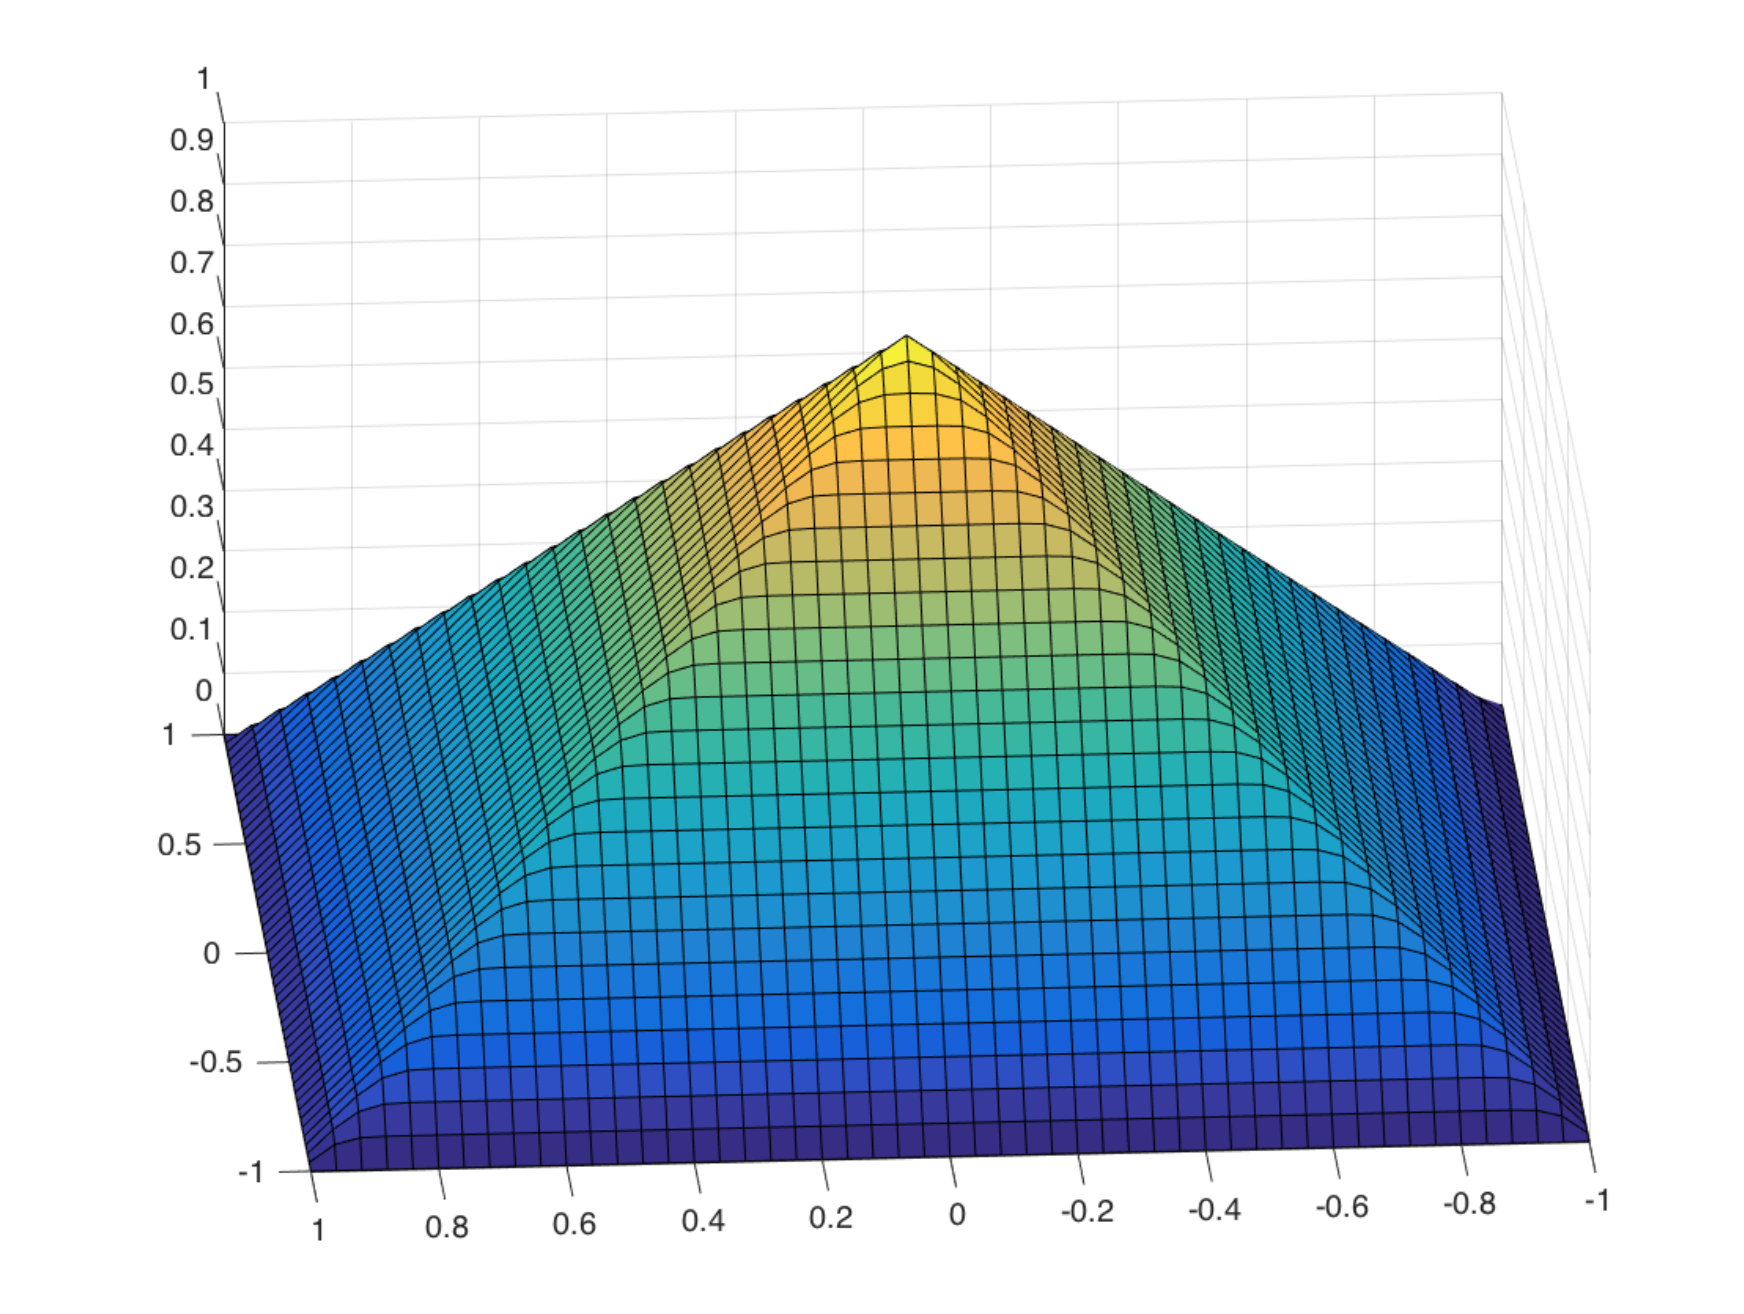
\includegraphics[scale = 0.4]{square.png}
	\caption{Solution in a square domain}
	\label{fig:3}
\end{figure}\\
\noindent
The profile shown in Figure \ref{fig:3} is the \textbf{Viscosity Solution} of the Eikonal Equation. A $50 \times 50$ grid was used to generate the profile till steady state with $\epsilon = 10^{-5}$. Some observations can be made from the solution shown in Figure \ref{fig:3}. The equation (\ref{eq:1}) does not accept solutions with a local minima (not a viscosity solution \cite{lions}). This gives an idea about how the solution should look like on other domains. For example, a right circlular cone is observed in the case of a circle and so on. \\

\noindent
Numerical Experiments were conducted using \textbf{Fortran90} to find out the order of convergence of the scheme with $\epsilon = 10^{-16} \approx$ Machine Error. The \textbf{inout} matrix for a circle with a $10 \times 10$ mesh is shown in Figure \ref{fig:4}
\begin{figure}[h!]
	\centering
	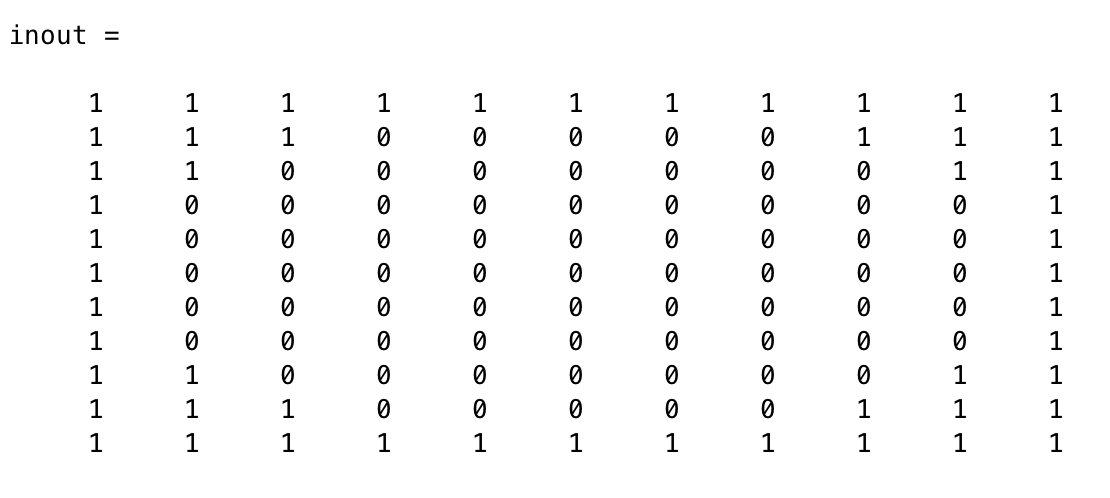
\includegraphics[scale=0.5]{inout.png}
	\caption{\textbf{Inout} Matrix for $10 \times 10$ mesh}
	\label{fig:4}
\end{figure}\\
\noindent
With this \textbf{inout} matrix, we compute the necessary distances near the boundary, for use in the Finite Difference Formula. Following is the profile, obtained when the Rouy and Tourin Scheme is run for $50 \times 50$ mesh on the master rectangle with steady state $\epsilon = 10^{-16}$.
\begin{figure}[h!]
	\centering
	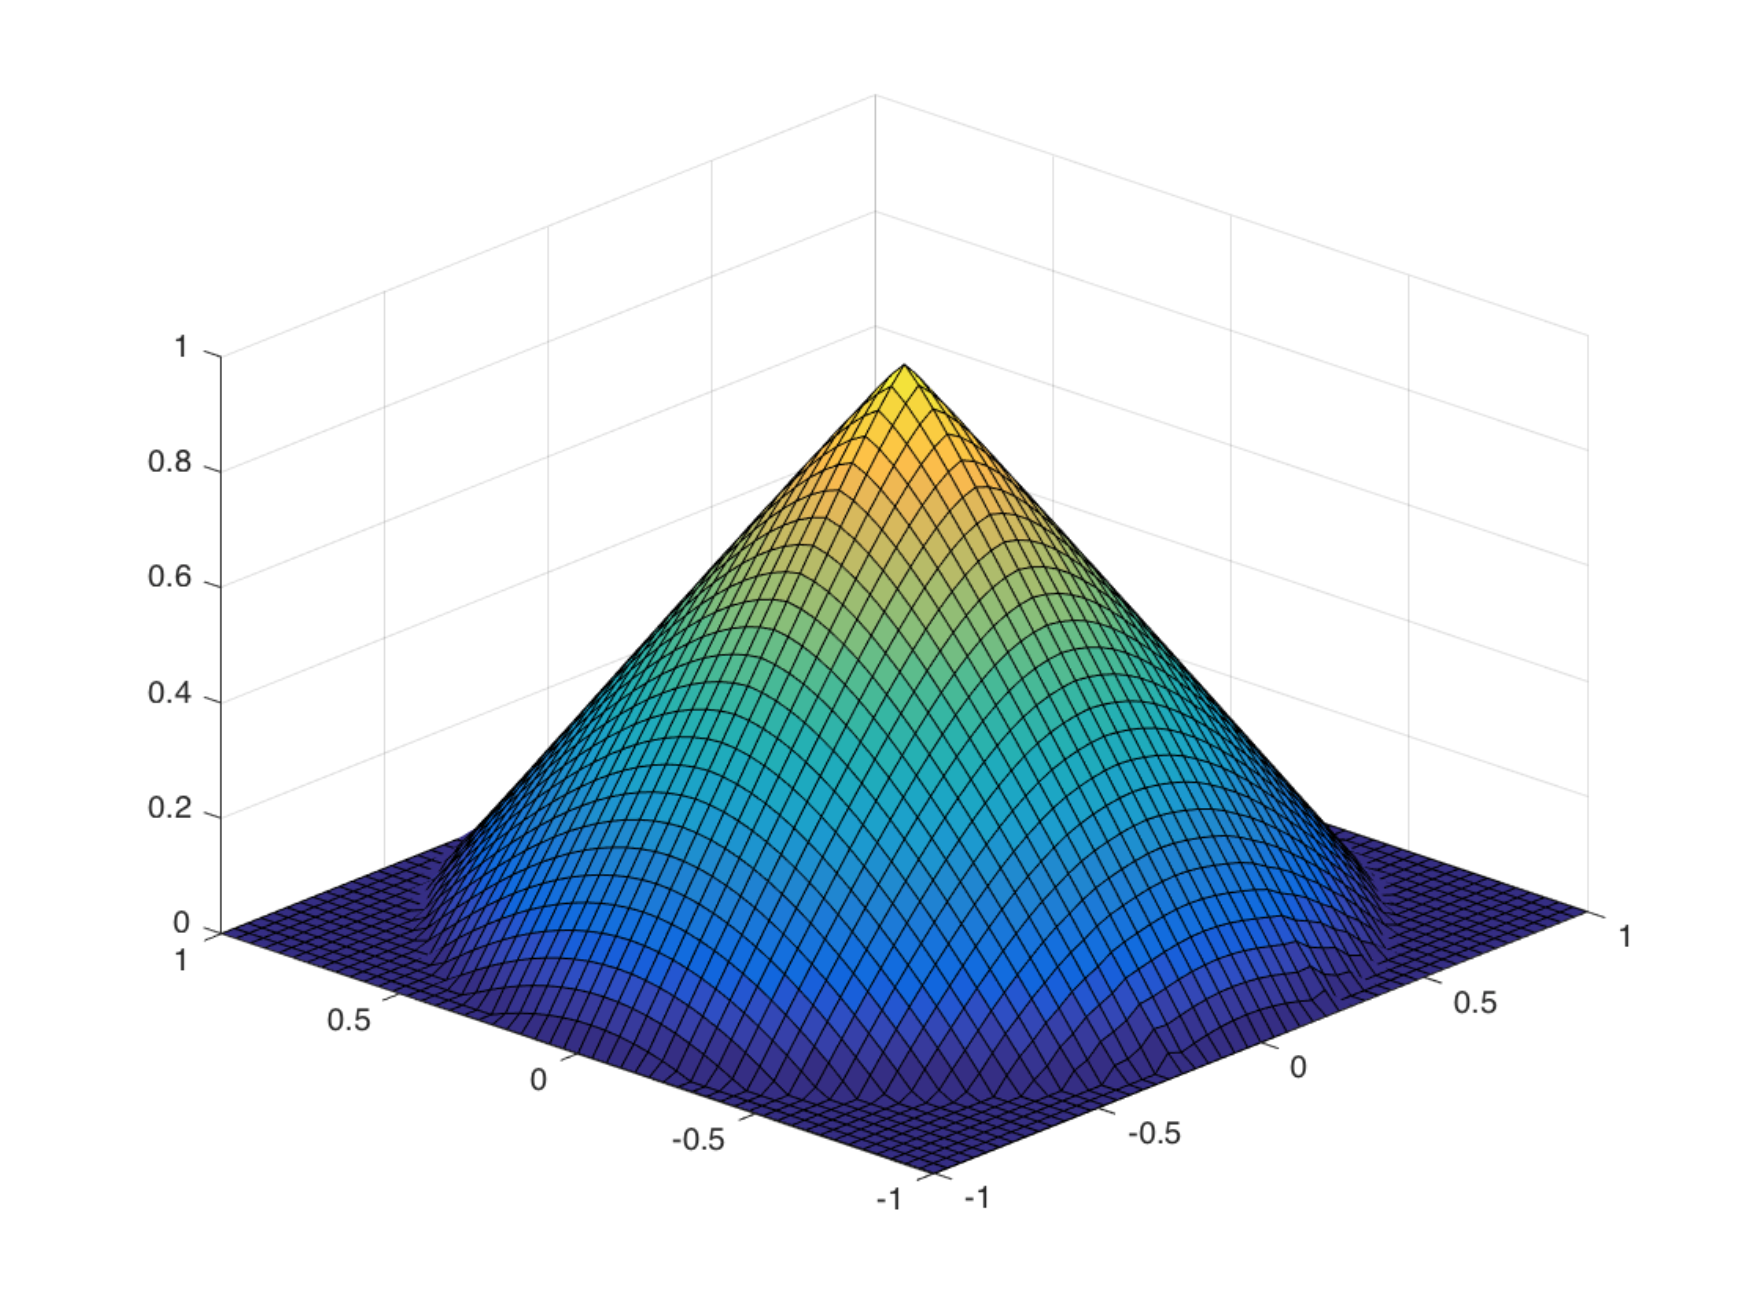
\includegraphics[scale = 0.3]{circle.png}
	\caption{Solution in a circular domain}
	\label{fig:5}
\end{figure}\\

\noindent
Using \textbf{Fortran90}, order of convergence analysis was performed on the scheme and the results are tabulated.\\
\begin{center}
	\begin{tabular}{|c|c|c|}
	\hline
	N & Error & Order of Convergence\\
	\hline
	10 & 0.9878E-01 & 0.685 \\
	\hline
	20 & 0.6145E-01 & 0.728 \\
	\hline	
	40 & 0.3710E-01 & 0.738 \\
	\hline	
	80 & 0.2223E-01 & 0.761 \\
	\hline	
	160 & 0.1311E-01 & 0.783 \\
	\hline	
	320 & 0.0762E-01 & 0.800  \\
	\hline
	640 & 0.0437E-01 & -\\
	\hline
\end{tabular}
\end{center}

\noindent
The same method can be used to generate profiles for a variety of domains as shown. The idea is to tweak the \textbf{inout} matrix corresponding to the shape of the domain and appropriately take care of the immersed boundary grid points.

\begin{figure}[h!]
	\begin{subfigure}{.5\textwidth}
		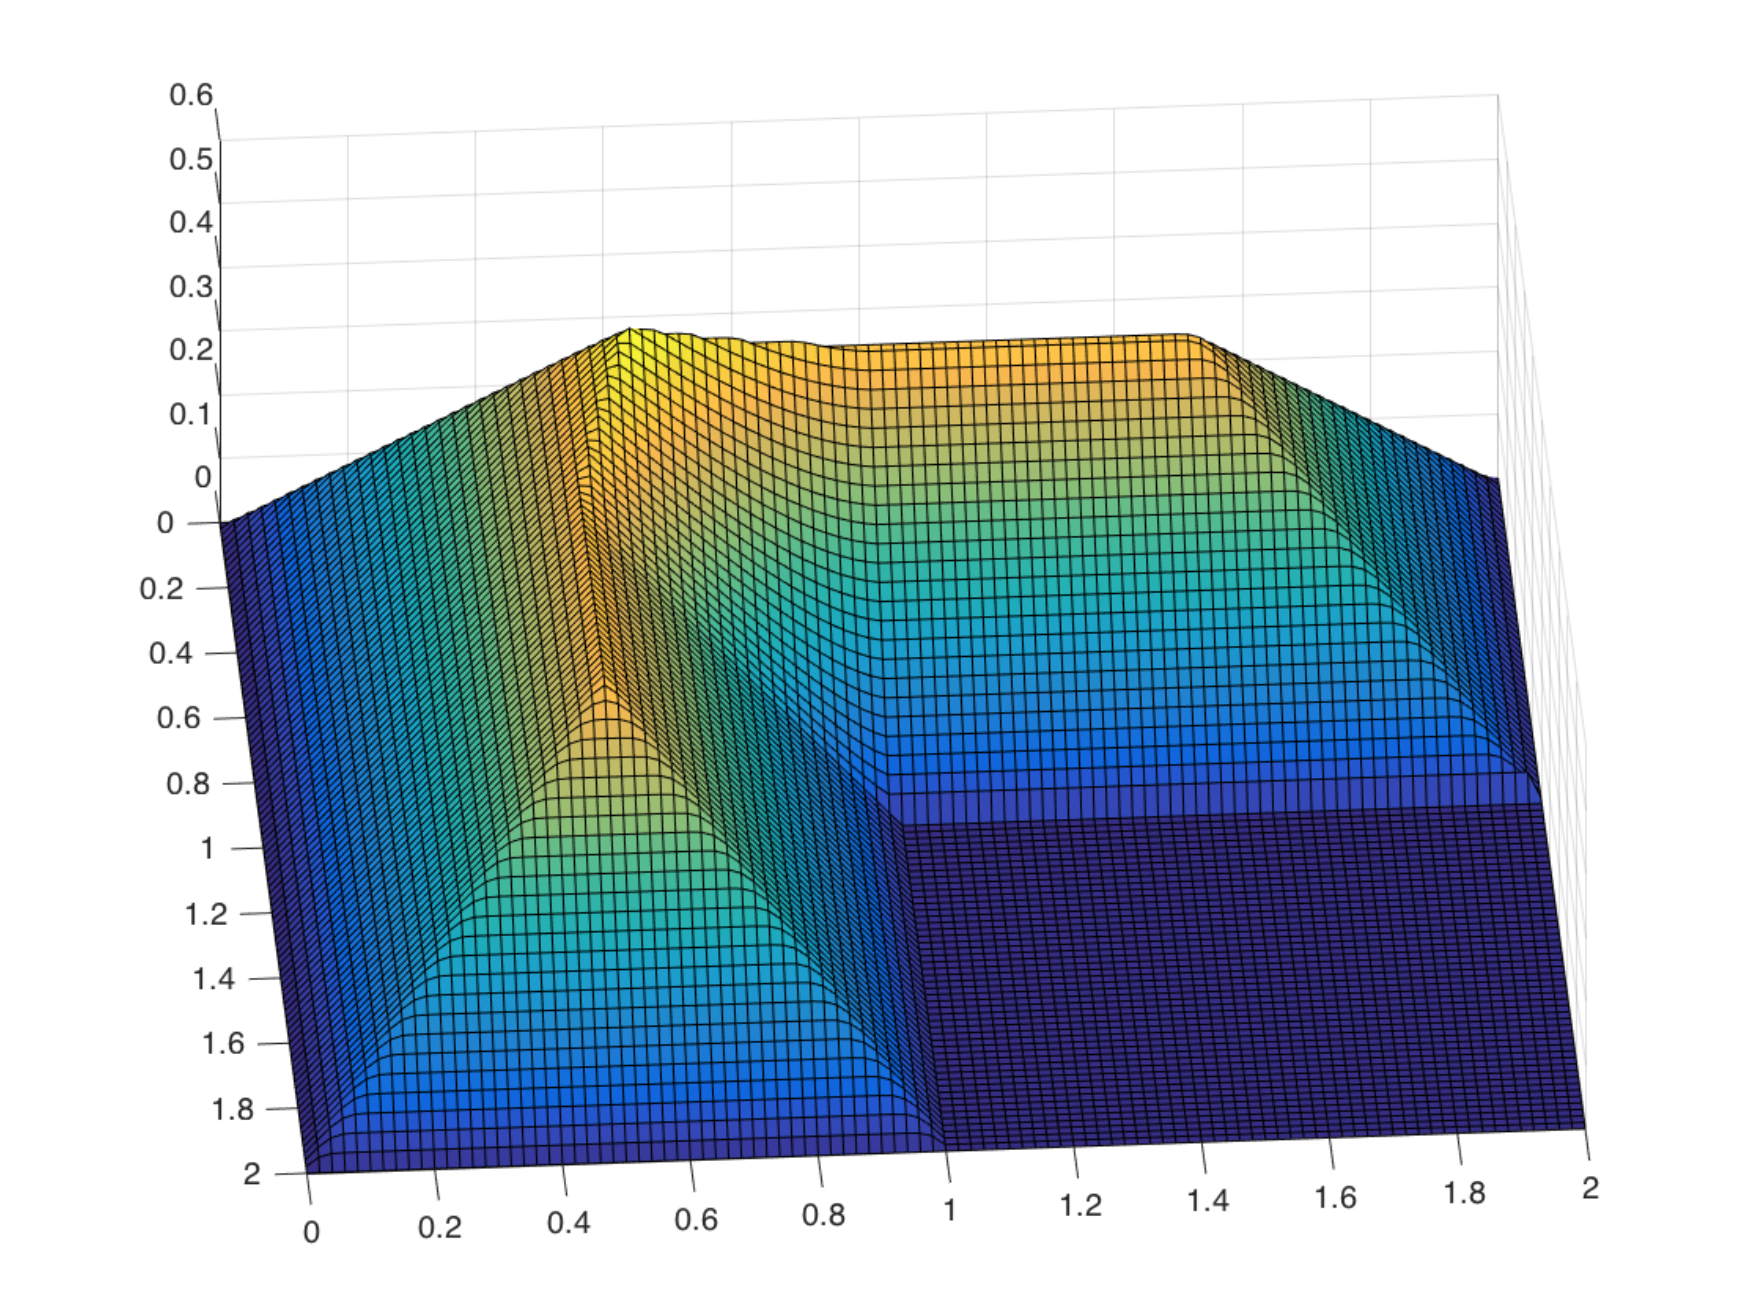
\includegraphics[scale = 0.2]{ldomain.png}
		\caption{L-Domain}
		\label{fig:6}
	\end{subfigure}
	\begin{subfigure}{.5\textwidth}
		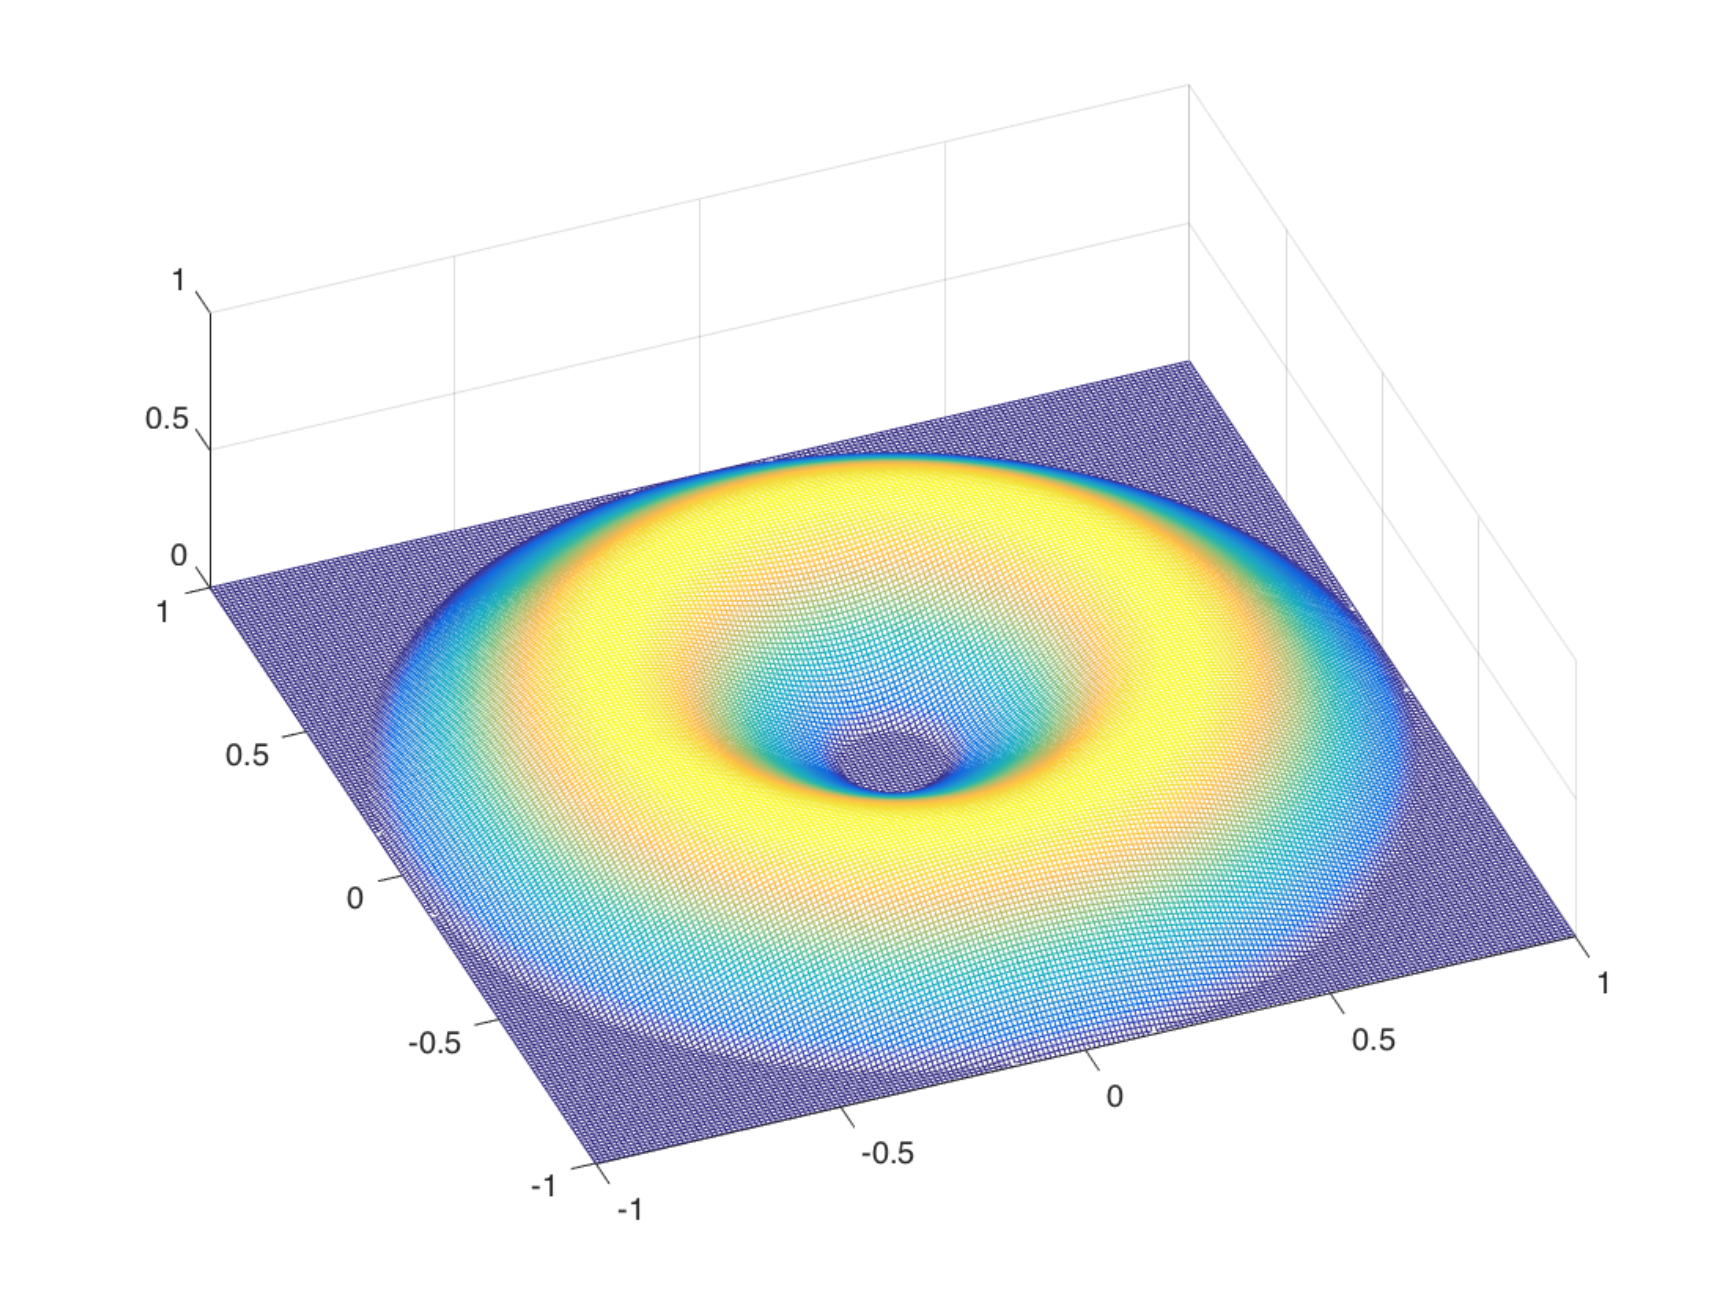
\includegraphics[scale = 0.2]{circlehole.png}
		\caption{Circle with a hole in the middle}
		\label{fig:7}
	\end{subfigure}
	\caption{Other Domains}
\end{figure}

\noindent
Figure \ref{fig:6} and Figure \ref{fig:7} shows the profile that is obtained when the Immersed Boundary Technique is applied to solve the Eikonal Equation on a L-Shaped Domain and a circle with a hole in it (non-convex domains) respectively. Similar Experiments can be conducted to model various problems in a variety of domains.

\chapter{Adaptive CFL condition for accelerating convergence}
Performance of the code can be improved by changing size of the time step used at each grid point. To increase the speed of computation, we use a higher value of $\Delta t$ at the interior (as the mesh parameter $h$ is larger and hence the limit on the time step $\Delta t$ is also higher) and lower value of $\Delta t$ on points near the boundary.\\

\noindent
With the update formula, 
\begin{equation}
	v_{i,j}^{n+1} = v_{i,j}^n - \Delta t (\dots
\end{equation}
we compute the solution at $t = t_{n+1}$  using $t = t_n$. Refer Figure \ref{fig:8}.\\
\begin{figure}[h!]
	\centering
	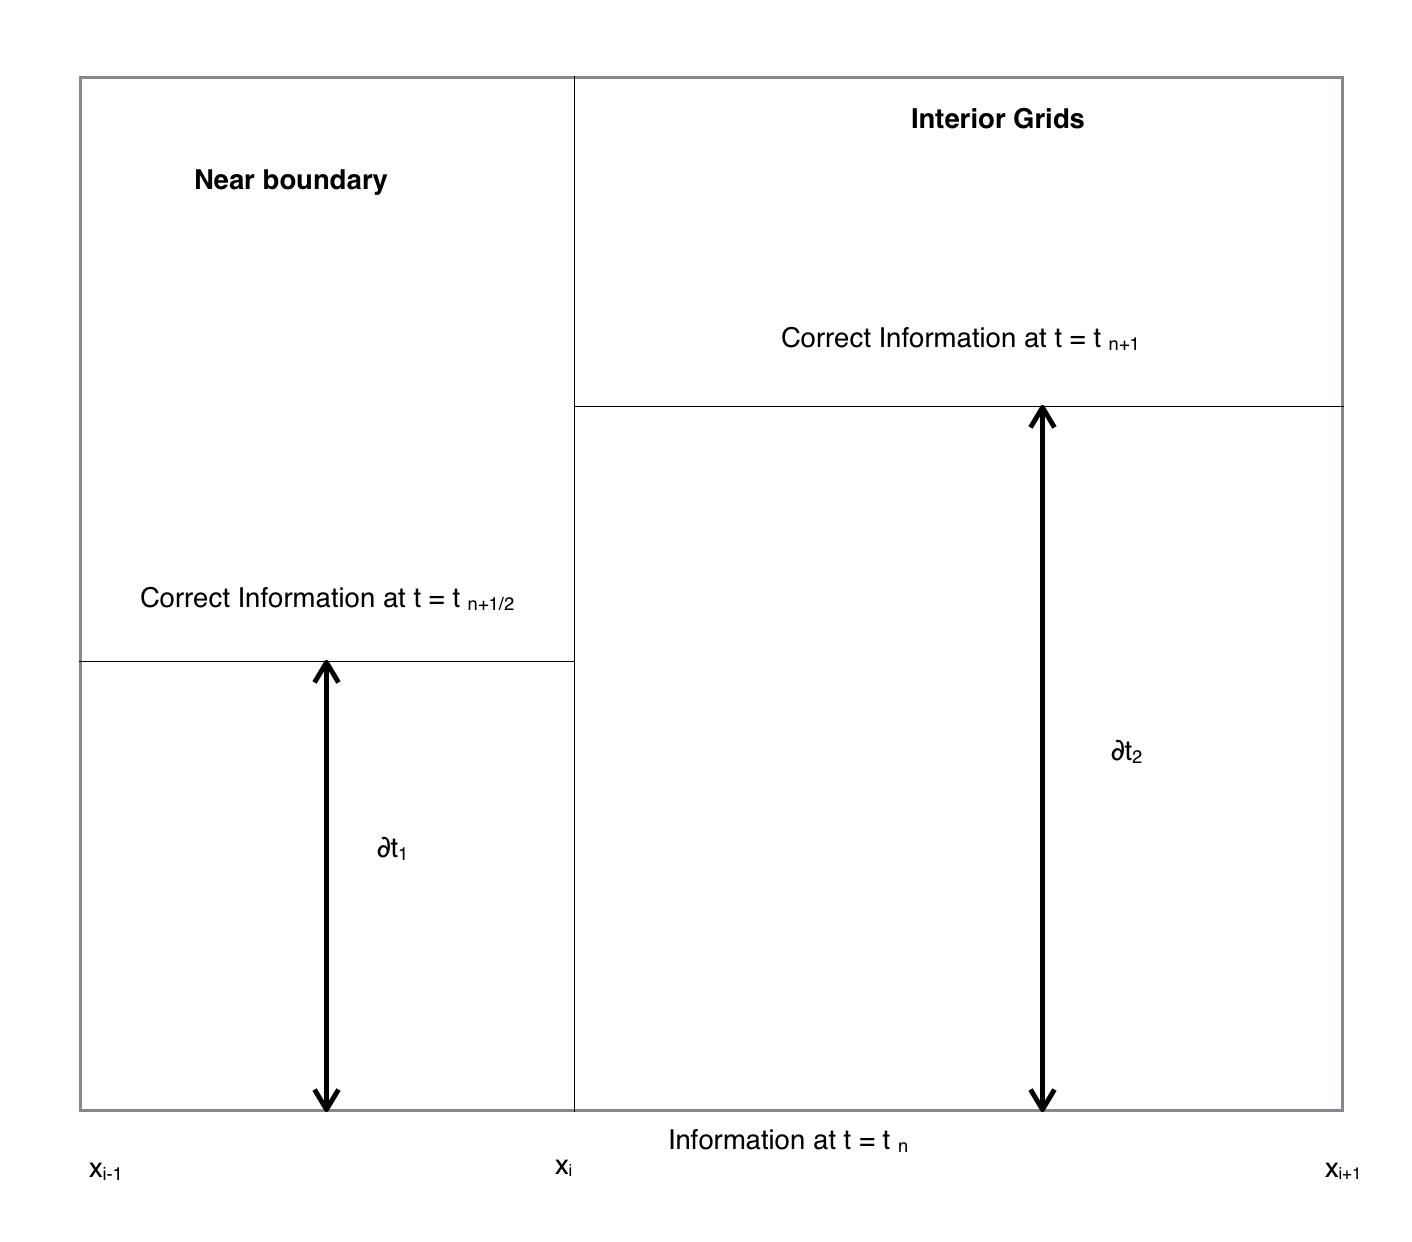
\includegraphics[width = 10cm, height = 6cm]{improv.png}
	\caption{Varying time steps}
	\label{fig:8}
\end{figure}

\noindent
We use the CFL Condition to find out the time step $\Delta t$ with respect to the mesh size $h$. The time step will be \textbf{larger} where the mesh is \textbf{coarse} and \textit{smaller} where the mesh is \textit{fine}. With this we march faster in time in the interior and march slowly in time near the boundaries. So, to compute the solution in $x_i$ (Rf. Figure \ref{fig:8}), we require information at $x_{i-1}$ and $x_{i+1}$ at all times.\\

\noindent
So the solution $u = u(x,y,t)$ will not give us the right result at a particular time $t$, because some grid points are evaluated at different times and the solution $u(x,y,t)$ would not make any sense. \\

\noindent
But as the information is correctly propogated over time $t \to \infty$, the solution is obtained as all the grid values would have reached the steady state, but with different speeds.\\

\noindent
We observe that the speed of computation has immensely improved and we were able to obtain the same order of convergence without the adaptive time stepping. 
\begin{center}
	\begin{tabular}{|c|c|c|}
		\hline
		N & Error & Order of Convergence\\
		\hline
		10 & 0.9878E-01 & 0.685 \\
		\hline
		20 & 0.6145E-01 & 0.728 \\
		\hline	
		40 & 0.3710E-01 & 0.738 \\
		\hline	
		80 & 0.2223E-01 & 0.761 \\
		\hline	
		160 & 0.1311E-01 & 0.783 \\
		\hline	
		320 & 0.0762E-01 & 0.800  \\
		\hline
		640 & 0.0437E-01 & 0.814 \\
		\hline
		1280 & 0.0249E-01 & 0.834 \\
		\hline
		2560 & 0.0139E-01 & - \\
		\hline
	\end{tabular}
\end{center}
\pagebreak
\subsection{Stability}
In this section, we discuss the stability of the finite difference scheme. For this we consider the 1D Advection Equation and this idea can be extended for the Eikonal Equation as well.
\begin{equation}
	u_t + u_x = 0
\end{equation}
Since the wave is propogating towards the right, we use the backward difference scheme.
\begin{equation}
	u_i^{n+1} = u_i^n - \frac{\Delta t}{h} \left( u_i^n - u_{i-1}^n \right)
\end{equation}

\begin{figure}[h!]
	\centering
	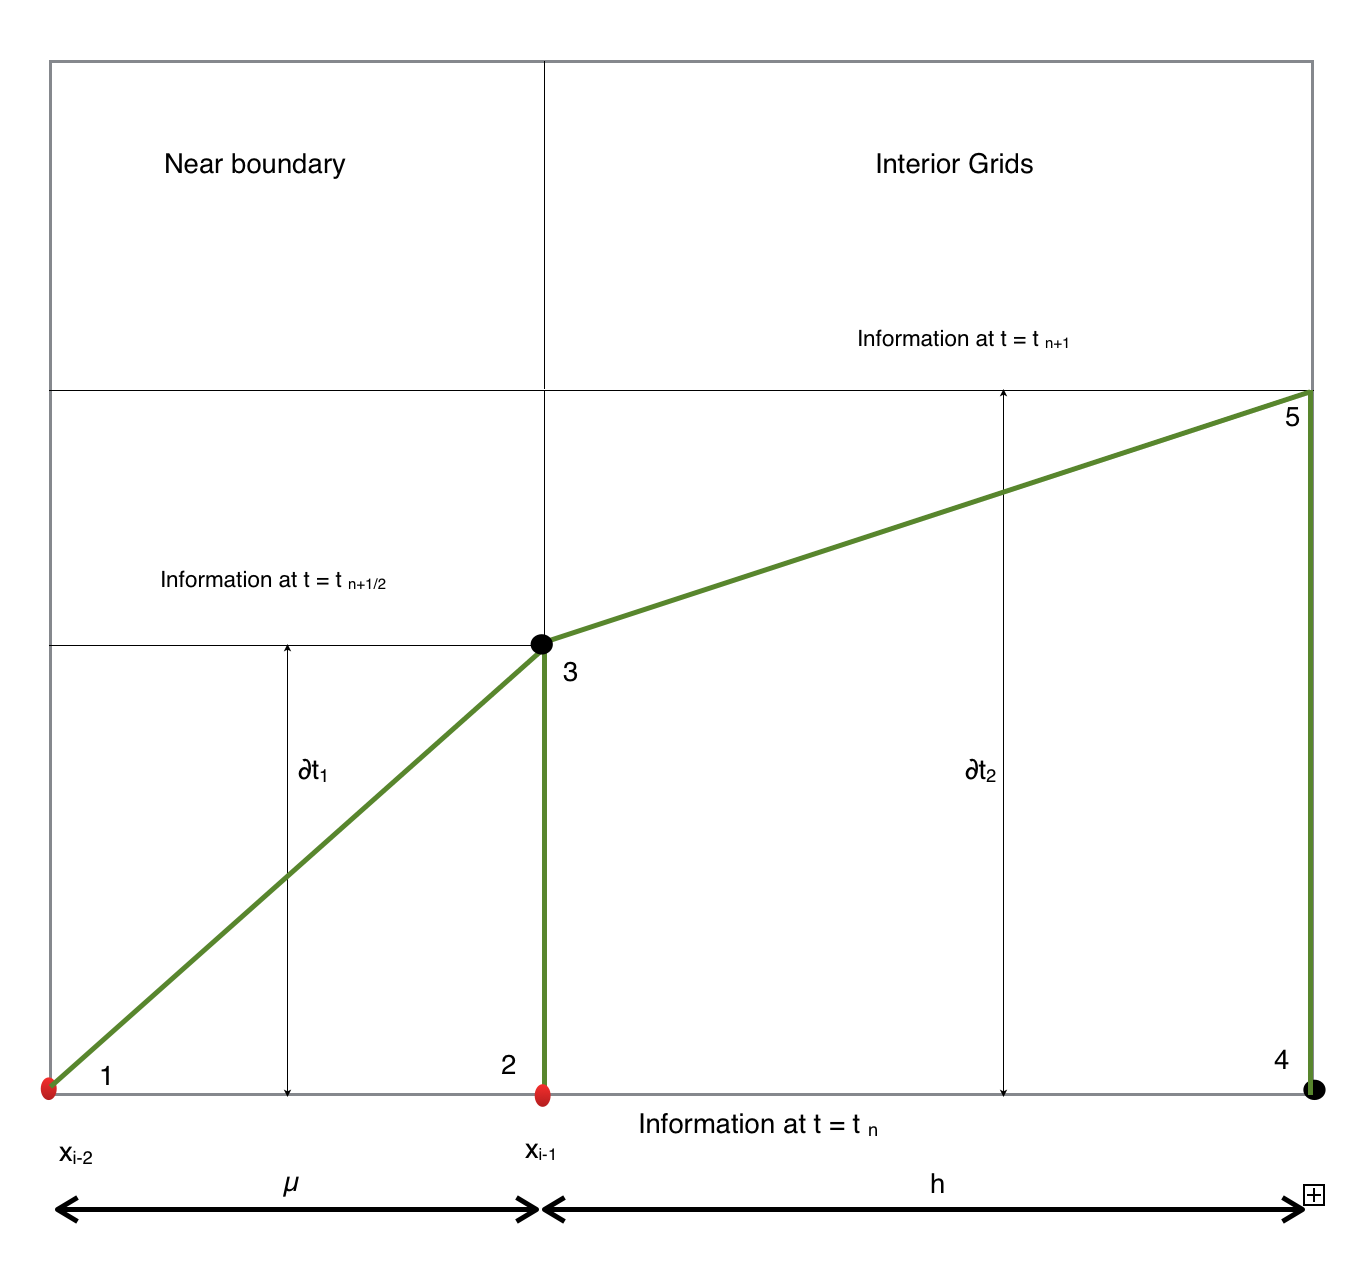
\includegraphics[width = 10cm, height = 8cm]{stencil.png}
	\caption{The Finite Difference stencil}
	\label{fig:9}
\end{figure}

\noindent
Now consider the finite difference stencil, shown in Figure \ref{fig:9}. The values of $v$ at points (1)-(5) is shown in the following table. For brevity, let us denote the value of $v$ at some $t$ in $[t_n, t_{n+1}] $ as $v_i^{n+\frac{1}{2}}$
\begin{center}
	\begin{tabular}{|c|c|}
		\hline
		Point & Value\\
		\hline
		1 & $v_{i-2}^n$ \\
		\hline
		2 & $v_{i-1}^n$ \\
		\hline
		3 & $v_{i-1}^{n+\frac{1}{2}}$ \\		
		\hline
		4 & $v_{i}^n$ \\
		\hline
		5 & $v_{i}^{n+1}$ \\				
		\hline
	\end{tabular}
\end{center}

\noindent
To find the values of $v_{i-1}^{n + \frac{1}{2}}$ and $v_i^{n+1}$ using the known $v_i^n$, $v_{i-1}^n$, $v_{i-2}^n$, we have the upwind scheme,
\begin{eqnarray}\label{eq:4}
	v_{i-1}^{n+\frac{1}{2}} &=& v_{i-1}^n - \frac{\partial t_1}{h} \left(v_{i-1}^n - v_{i-2}^n\right)\\\label{eq:5}
	v_i^{n+1} &=& v_i^n - \frac{\partial t_2}{h} \left(v_i^n - v_{i-1}^{n+\frac{1}{2}}\right)
\end{eqnarray} 

\noindent
Combining (\ref{eq:4}) and (\ref{eq:5}), we have,
\begin{equation}
	v_i^{n+1} = v_i^{n} - \frac{\partial t_2}{h} \left(v_i^n - \left(v_{i-1}^n - \frac{\partial t_1}{h} \left(v_{i-1}^n - v_{i-2}^n \right) \right) \right)
\end{equation}
\noindent
Rearranging,
\begin{eqnarray}
	v_i^{n+1} &=& \left(1-\frac{\partial t_2}{h}\right) v_i^n + \left(1-\frac{\partial t_1}{h}\right) \left(\frac{\partial t_2}{h}\right) v_{i-1}^n + \left(\frac{\partial t_1}{h}\frac{\partial t_2}{h}\right) v_{i-2}^n\\
	\implies v_i^{n+1} &=& H(v_{i-2}^n, v_{i-1}^n, v_{i}^n)
\end{eqnarray}
\noindent
For the scheme to be monotone ,$H$ must be non-decreasing in each of its variable. If we check for the same, we get
\begin{eqnarray} \nonumber
	\partial t_1 \le h \\\nonumber
	\partial t_2 \le h
\end{eqnarray}

\noindent
Combining these two we have the monotonicity condition.
\begin{equation}
	\max(\partial t_1, \partial t_2) \le h \label{eq:7}
\end{equation}

\noindent
The scheme is consistent and from (\ref{eq:7}), we can say that the scheme is convergent to the exact solution.


\nocite{*}
\bibliographystyle{acm}
\bibliography{biblio}
\end{document}
